% !TEX root = thesis.tex
\chapter{Introduction}

\begin{quote}
Design is not just what it looks like and feels like. Design is how it works.

--- Steve Jobs
\end{quote}

Our environment is replete with products that have dedicated physical user interfaces like game controllers, musical instruments or personal medical devices. While the ubiquity of smart phones has led to a rise in touchscreen applications, retaining physicality has important benefits such as tactile feedback and high performance manipulation \cite{klemmer-bodies}. For example, gamers prefer physical input for speed and performance, musicians for virtuosity and control. Rapid additive manufacturing technologies enable designers and makers (henceforth we refer to both groups jointly as ``makers'') to quickly turn CAD models of such future devices into tangible prototypes. While such printed form prototypes can convey the look and feel of a physical device, they are fundamentally passive in that they do not sense or respond to manipulation by a user. Building integrated prototypes that also exhibit interactive behavior requires adding electronic sensing components and circuitry to the mechanical design (see Figure \ref{fig:3dcases}).

\begin{figure}
\centering
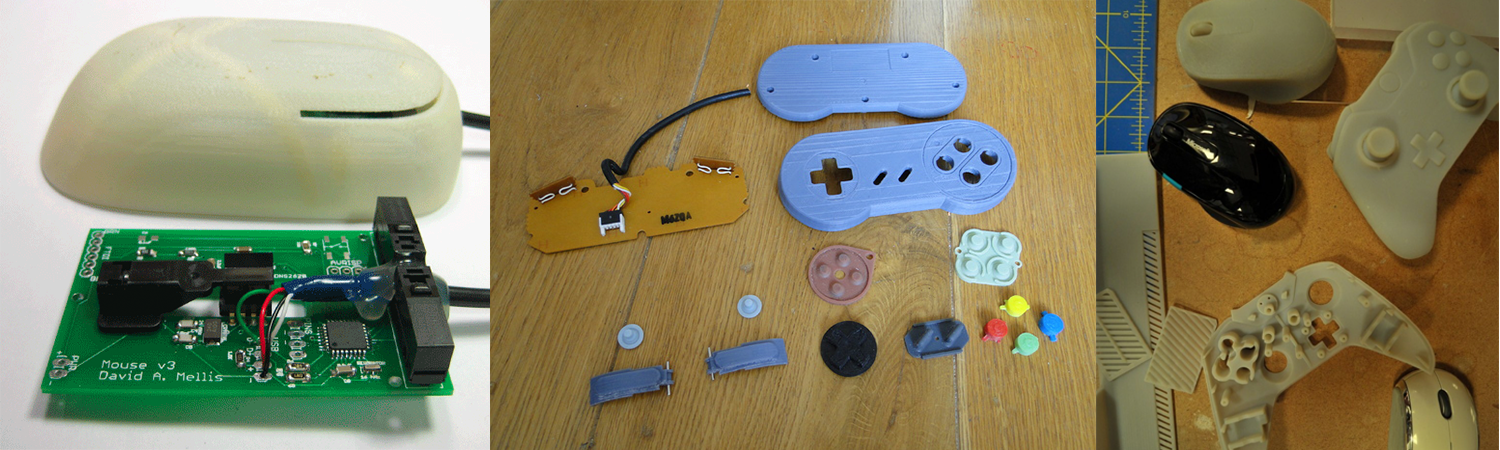
\includegraphics{figures/3dcases.png}
\caption{Makers use 3D printing to explore case form factors for interactive objects, like Dave Mellis's mouse (left) or Thingiverse author srepmub's game controller (center). Even professional designers like those at Microsoft use 3D printing for form-finding (right). However, this technique requires two separate processes: designing the case, then designing the functionality, typically in the form of circuitboards.}
\label{fig:3dcases}
\end{figure}

Existing research has developed electronic toolkits that lower the threshold of making physical prototypes interactive \cite{arduino,greenberg-phidgets}. However, such toolkits still require makers to manually assemble printed parts and sensors. Such assembly may also require significant changes to a 3D model (e.g., to add fasteners or split an enclosure into two half shells). Detailed electro-mechanical co-design is time-consuming and cumbersome and mismatched with the spirit of rapid prototyping. Alternatively, makers may instrument their  \emph{environments} with sensors \cite{akaoka-displayobjects,wilson-depthtouch} to add interactivity, but these approaches limit interactive testing to the lab in small, restricted areas.

\emph{We aim to uncover the most cost-effective, fast, and flexible ways of sensing rapid-prototyped input devices.} This suggests several requirements:
\begin{enumerate}
\item \textbf{cost-effective} : we substitute commodity sensors available in laptops and smartphones for custom electronic parts where possible. We focus on \emph{single-sensor} techniques, where sensing of multiple user inputs can be achieved by affixing a sensing apparatus to a single point.
\item \textbf{fast} : fabrication and assembly of senseable devices should not take significantly longer than comparable passive devices, and necessary digital modifications should be performed automatically when complex or be reduced to templates when simple.
\item \textbf{flexible} : the means of sensing a prototype object should not impose undue burden on the physical designs of that object. Sensing techniques should accommodate a wide variety of input types (e.g., buttons, sliders, and dials) and body types (e.g., convex, concave, 3D).
\end{enumerate}
We propose a novel way of ensuring these properties: users create digital design files, which our tools modify automatically based on knowledge of the sensing technique that will ultimately be used. Users then fabricate their modified models using digital fabrication machines. Because the physical models are precisely fabricated based on the digital design files, this process creates a \emph{link between the digital and physical models}. Post-fabrication, we leverage this link to inform sensor processing: this allows us to \emph{avoid training} and/or \emph{improve sensing} for the interactive prototype.

\section{Contributions}

This thesis explores the realm of physically prototyping tangible input devices using digital fabrication machines. We have built several prototype design and sensing systems designed to test different parts of the design space. Thus, this thesis makes the following contributions:

\begin{enumerate}
\item Fabbing to sense: a model and sensing co-design technique which uses knowledge of a particular sensing paradigm to automatically modify digital design files before fabrication, allowing improved or training-free sensing of the fabricated prototype. We offer three exemplars of this technique: Midas, Lamello, and Sauron.
\item Midas, a method for automatically generating custom capacitive touch sensors---cut from adhesive-backed conductive foil---by synthesizing sensor pads and routing connections from a high-level graphical specification:
%which allows a designer to author a high-level graphical specification of an object---and from that creates custom-shaped, flexible capacitive touch sensors by synthesizing sensor pads, auto-routing connections, and generating instructions for assembly and use: 
\begin{enumerate}
    \item a design tool using this method to enable users to to fabricate, program, and share touch-sensitive prototypes
    \item an evaluation demonstrating Midas’s expressivity and utility to designers
    \end{enumerate}
\item Lamello, a technique using passive plastic tine structures, 3D printed at interaction points and with predictable vibrational frequencies, to create passive tangible inputs sensed via audio:
%a technique which integrates algorithmically-generated audio-producing tine structures into movable components, creating passive tangible inputs---sensed by a microphone which classifies the tine-generated audio---that do not require training examples for accurate sensing:
\begin{enumerate}
    \item a design pipeline which predicts tine frequencies (and an evaluation that they can be accurately predicted) and senses user manipulation of components in real time
    \item a discussion of information encoding techniques useful for this technique, and a series of scripts to generate parts utilizing these encodings
    \end{enumerate}
\item Sauron, a design tool enabling users to rapidly turn 3D models of input devices into interactive 3D printed prototypes where a single camera senses input: %\valkyrie{this is the clearest description. modify others to be like this!}
\begin{enumerate}
    \item a method for tracking human input on physical components using a single camera placed inside a hollow object
    \item two algorithms for analyzing and modifying a 3D model’s internal geometry to increase the range of manipulations that can be detected by a single camera.
    \item an informal evaluation of our implementation of these techniques usable on models constructed in a professional CAD tool.
    \end{enumerate}
\end{enumerate}

\section{Dissertation Sketch}

This section presents a brief sketch of the structure of this dissertation by chapters.

This dissertation first investigates the capabilities of modern digital fabrication machines and discusses single-sensor techniques compatible with those capabilities. Second, a solid foundation of related work is laid out. We then discuss three instances of analysis and design tools that help users design, fabricate, assemble, and \emph{use} input devices sensed in a variety of ways; for each technique we demonstrate its flexibility for use in many types of input devices. Finally, we conclude with suggestions for future work.

\subsection{Fabrication \& Sensing (Chapter 2)}

This chapter explores modern digital fabrication machines and the properties that can be employed in objects they fabricate. We additionally enumerate properties that can be realized by different types of machines.

Chapter 2 discusses single-sensor techniques compatible with those capabilities, as well as what makes each technique promising. Again, we focus on techniques which require a single sensing apparatus attached to a single point on an object. For example, we discuss the potential combination of 3D printed conductive metal with Hall effect sensors; inducing a current through the object could create a magnetic field detectable by the sensors. Also, we describe digitally fabricated paper combined with humidity/moisture sensors; especially for exertion-based interfaces, user interaction over time could cause the interface to collect and detect sweat. This thesis ultimately selects a few points to further examine in this space, described in Chapters 4-6.

\subsection{Related Work (Chapter 3)}

We situate this thesis in the realm of what's been done. In general, we draw heavily on work from four major traditions: graphics and optimization, sensing digitally-fabricated devices, modeling 3D objects, and creating prototypes.

\subsubsection{Graphics/Optimization}
The optimization community embraced digital fabrication early: they provide some of the earliest research on using pre-fabrication simulation to ensure good coverage from robotic spray heads without occlusion from model features \cite{gursoz-noodles}, or to account for deformities from specific printing processes \cite{hsu-numerical}. More recently, computer graphics researchers have leveraged pre-print simulation of multi-material printers to control post-print deformation behaviors \cite{bickel-deformation} and appearance \cite{lan-appearance}. We, too, perform pre-print simulation and optimization of 3D models, but for the purpose of creating \emph{interactive} objects.

\subsubsection{3D CAD Tools}
Many professional tools for 3D modeling exist \cite{solidworks, rhino}, and they serve their target users well. Researchers have made significant strides in inventing new styles of more accessible interactions for 3D modeling, for example by capturing users' hand-carving processes and convering them to toolpaths \cite{willis-interactive} or scanning, augmenting, and reproducing clay models \cite{savage-mmarks}. For the purposes of our investigations in this thesis, we created design tools to help author objects compatible with our sensing techniques: they are a complement to, rather than a replacement for, existing CAD tools research.

\subsubsection{Sensing Digitally-Fabricated Devices}
Sensing forms a key component of interactive devices, and thus has been significantly explored in the past. One common technique for sensing objects uses machine learning and guided manual training to detect interactions using sound \cite{ono-touchandactivate,laput-acoustruments}, capacitance \cite{sato-touche} or other signals. Our techniques focus on sensing done without machine learning, and often without any training at all. Inspired by ``Sensing Through Structure'' \cite{slyper-structure}, we design objects whose properties we know, which can inform how we sense them.

\subsubsection{Prototyping Tools}
Abundant research has examined questions around the types of prototypes that designers build in the course of designing a new object \cite{houde-prototypes}. Other work looks further into more facile ways of creating electronic and functional, for example using snap-together circuits \cite{littleBits, hartmann-dtools, villar-gadgeteer} or smart circuit substrates \cite{villar-voodooio}. One important limitation of these investigations is that they are limited to a constrained library of manufactured components: designers must make do with what they can buy. We conversely focus on customizable inputs that can be configured exactly as a designer wants them. Once an object is assembled, its functionality must be defined. We leverage techniques like programming by demonstration \cite{myers-pbd, hartmann-dtools} to help users define their objects' interactivity.

%% \valkyrie{bjoern's these are really long... how long do they need to be??}

\subsection{Midas: Capacitive Sensing of Custom 2D Layouts (Chapter 4)}

Our first exploration examines fabrication of 2D conductive materials sensed capacitively. Midas pushes towards a world in which prototyping physical interactive devices is as easy as prototyping GUI devices. Midas's sensing is capacitive, building on the popular capacitive touch sensing built in to smart phones and other touch-screen devices, but it explores how to prototype touch-based interactions where input and output are \emph{not} co-located, as they are on touch screens. Designers are given a drag-and-drop authoring system to create capacitive touchpads on the surface of objects, and from these designs generates 2D design files for fabrication. These files can then be cut from a conductive material and sensed using an automatically-configured microcontroller board. Midas also offers support for programming the input devices designed via PBD and websockets.

\begin{figure}
\centering
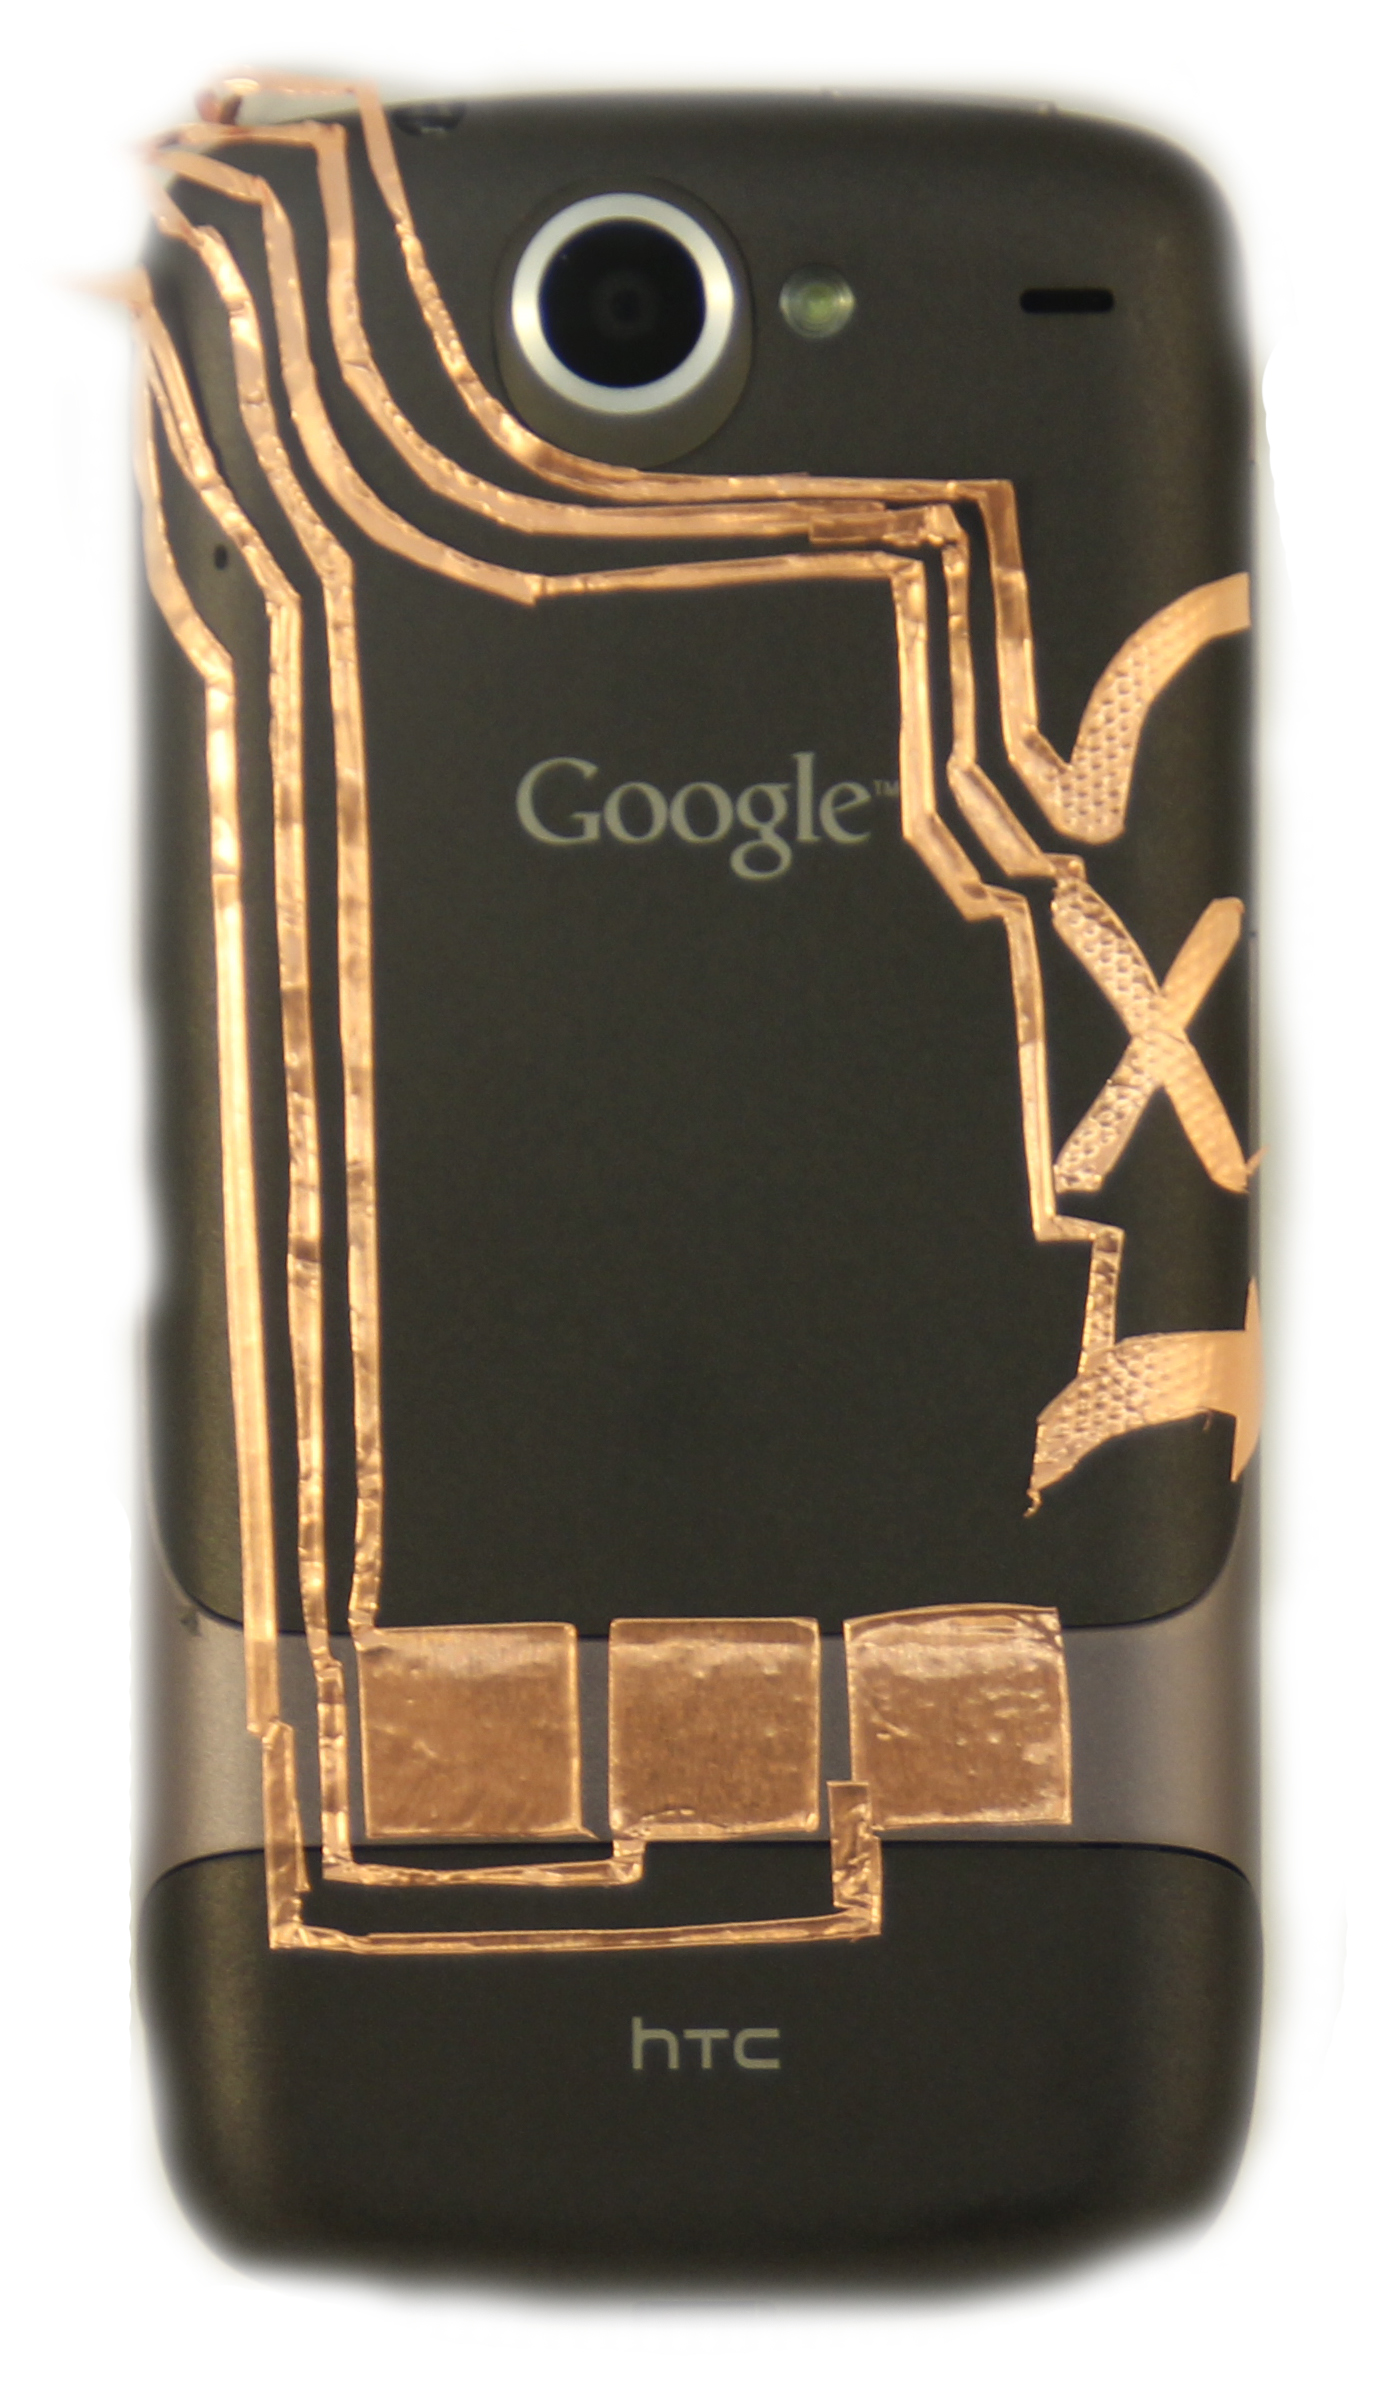
\includegraphics[width=2in]{figures/midas/midas-intro.jpg}
\caption{A Midas-generated interface with buttons for checking email mounted on the back of a smart phone.}
\label{fig:midas-intro}
\end{figure}

The advantages of capacitive sensing in this manner are numerous. It can be deployed on any flat, ruled, or developable object's surface (see Figure \ref{fig:midas-intro}). The sensors are cheap and easy to fabricate---whether on a vinyl cutter, using a circuitboard mill, or in inkjet printed conductive ink. Sensor assembly is \emph{fast}: users simply need to attach the sensor dongle's wires to their fabricated sensor pads (e.g., using tape).

In this chapter, we will detail Midas's implementation, as well as discussing possible uses, drawbacks of the current system, and work for the future.

\begin{figure}
\centering
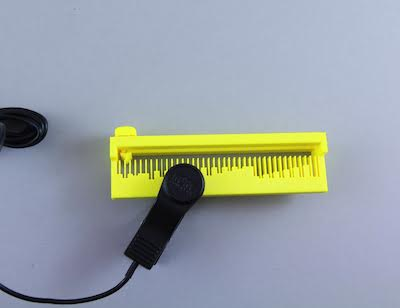
\includegraphics[width=3in]{figures/lamello/lamello-intro.jpeg}
\caption{A Lamello-based interface with a series of plastic tines on a slider, which can be classified by the attached contact microphone.}
\label{fig:lamello-intro}
\end{figure}

\subsection{Lamello: Acoustic Sensing of 2D/3D Mechanisms (Chapter 5)}

Second, this thesis dives into an examination of acoustic-based sensing for devices fabricated in 2D, 3D, or a combination. The Lamello project investigates the use of tine-like structures for repeatable and predictable audio frequency generation. These tines can be printed at interaction points (e.g., under the path of a human input slider) such that they are struck when a user manipulates input components. The mechanical vibrations created by striking the tines can be detected with a contact microphone and classified using frequency analysis (see Figure \ref{fig:lamello-intro}).

Leveraging uniform 2D lasercut or 3D printed plastics as sound-creating input devices offers flexibility to designers with different levels of access to fabrication machines. In addition, beyond Midas's offering of flat input surfaces activated by a simple touch, Lamello explores input mechanisms that users can push, slide, and turn. The technique of passive audio generation for sensing also opens up opportunities in the future Internet of Things: multiple unpowered Lamello-type input devices may be placed in the environment and sensed by a single microphone, perhaps located on a laptop or smartphone.

This chapter details our experiments confirming that our 3D-printed tine structures behave in predictable ways in spite of the non-uniform nature of the materials that comprise them. We also discuss, using several exemplars, techniques for integrating the tines into existing input component designs. Further, we describe information encoding principles for tine generation.

\subsection{Sauron: Vision-Based Sensing of 3D Printed Mechanisms (Chapter 6)}

Finally, we explore full 3D input devices sensed using computer vision. Sauron is a design and sensing toolkit for creating 3D printed input devices---which can include components like joysticks or dials---sensed with a single embedded camera. The Sauron tool makes automatic modifications to allow for this sensing, reconfiguring the \emph{interior} parts of the inputs and performing interference simulation (see Figure \ref{fig:sauron-intro}).

\begin{figure}[h]
\centering
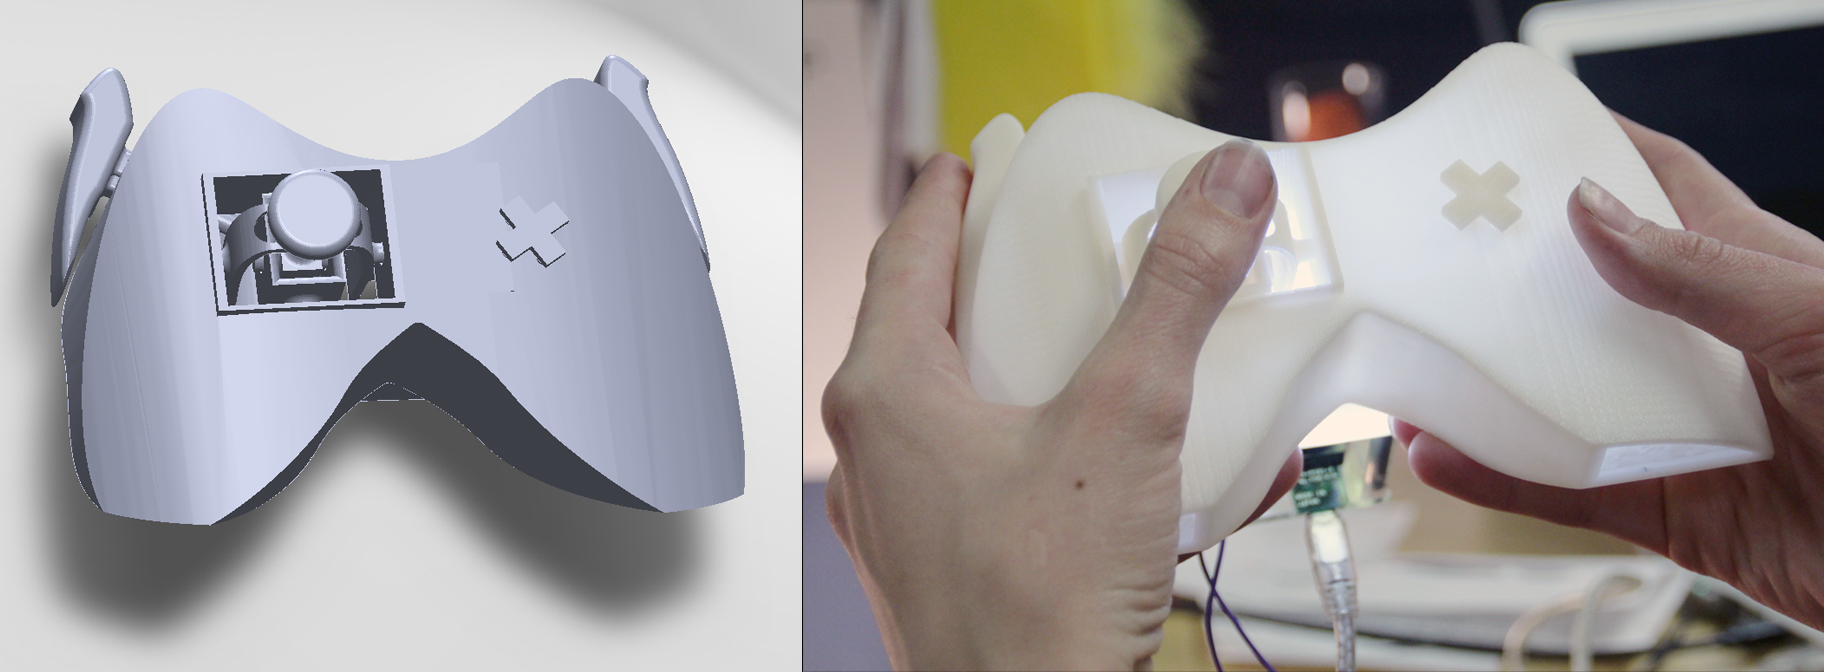
\includegraphics[width=4in]{figures/sauron/fig1-gamecontroller.jpg}
\caption{A Sauron-optimized game controller with a joystick, a direction pad, and several buttons.}
\label{fig:sauron-intro}
\end{figure}

Sauron's interfaces have additional flexibility over those for Midas or Lamello: they allow \emph{continuous} sensing of user input. They can be fabricated on any 3D printer which can generate support material, and the pre-fabrication simulation process relies only on geometry rather than any particular materials properties for its processing. %\valkyrie{not sure what else to put here...}

In this chapter we describe our implementation of Sauron as a plugin for a commercial CAD tool, as well as the vision sensing code we built. Finally, we elaborate on limitations of the current system and places we may improve it, as well as future work in the area.

\subsection{Conclusion \& Future Work (Chapter 7)}

The final piece of this thesis reviews the contributions described and re-evaluates assumptions made in the projects constituting its main chapters. Namely, our projects leverage a \emph{single fabrication machine} for creating \emph{one prototype} at a time, which is \emph{hand-optimized} by a designer and sensed by a \emph{single} sensor. Re-evaluating these leads to interesting pointers for future work in cooperation among fabrication machines, branching prototypes, machine-optimized prototype designs, and usage of combination sensors that can still be mounted at a single point.

\section{Statement of Multiple Authorship and Prior Publication}

The research presented in this dissertation was not undertaken by me alone. While I initiated
and led all projects described herein, I must acknowledge the contributions of my talented group of collaborators: without their efforts, this research could not have been realized in its current scope.

In particular, Midas's routing features were implemented by Xiaohan Zhang, and the video was created by Lora Oehlberg. Andrew Head performed much debugging and audio testing on the Lamello project, and that project benefited from the wisdom of my collaborators Dan Goldman (who provided the initial idea), Gautham Mysore, and Wilmot Li at Adobe. Sauron's computer vision was implemented by Colin Chang, and many thanks are due Mark Oehlberg for assisting in the creation of the necessary circuitboards for that project.

My advisor, Bj\"orn Hartmann, provided invaluable advice and guidance on all projects detailed in this document.

This dissertation is partially based on papers previously published in ACM conference proceedings; I am the primary author on all publications. In particular, Midas was published at UIST 2012 \cite{savage-midas}; Lamello at CHI 2014 \cite{savage-lamello}; and Sauron at UIST 2013 \cite{savage-sauron}.